%
% j1a SwapForth manual
%

%\documentclass[letterpaper, 10 pt, conference]{ieeeconf}  % Comment this line out
                                                          % if you need a4paper
%\documentclass[onecolumn,a4paper, 10pt, conference]{ieeeconf}      % Use this line for a4
\documentclass[10pt]{book}

\usepackage[paperwidth=6.69in, paperheight=9.61in]{geometry}

% \usepackage[T1]{fontenc}
% \usepackage[scaled]{helvet}
% \renewcommand*\familydefault{\sfdefault}

\usepackage{lmodern}

% \usepackage[T1]{fontenc}
% \usepackage[urw-garamond]

% See the \addtolength command later in the file to balance the column lengths
% on the last page of the document

\usepackage{makeidx}         % allows index generation
\makeindex
\usepackage{graphicx}        % standard LaTeX graphics tool
                             % when including figure files
\usepackage{multicol}        % used for the two-column index
% \usepackage[bottom]{footmisc}% places footnotes at page bottom
\usepackage{amsmath}
\usepackage{longtable}
\usepackage{color}
\usepackage{fancyvrb}
\usepackage{rotating}
\usepackage{supertabular}
\usepackage{bytefield}
\usepackage{url}
\usepackage{array}
\usepackage{verbatim}
\usepackage{setspace}
\usepackage[]{caption}
\usepackage{listings}
\usepackage{wrapfig}
\usepackage{framed}
\usepackage{alltt}
\captionsetup{font=small}

% The following packages can be found on http:\\www.ctan.org
\usepackage{graphics} % for pdf, bitmapped graphics files
\usepackage{epsfig} % for postscript graphics files
\usepackage{tikz}
\usetikzlibrary{arrows,decorations.pathmorphing,backgrounds,positioning,fit,petri,shapes.misc}
\usepackage[linkbordercolor={.9 .9 .9}]{hyperref}

\usepackage[dotinlabels]{titletoc}

\newlength\widest
\settowidth\widest{99.99.}

\titlecontents{section}[1pc]
{\addvspace{0pc}}
{\parbox[t]{\widest}{\hfill\thecontentslabel.}
\hspace{3mm}}
{}
{\normalsize\titlerule*[6pt]{.}\contentspage}
[\addvspace{0pt}]

% Customizations for this document only
\definecolor{light-gray}{gray}{0.90}

\newcommand{\gdtwo}{Gameduino 2 }
\newcommand{\gdtwos}{Gameduino 2's }
\newcommand{\itwoc}{I$^{\textrm{2}}$C }

\newcommand{\png}[1]{
\begin{center}
\includegraphics[width=0.8\textwidth]{assets/#1.png}
\end{center}
}

\newcommand{\szpng}[2]{
\begin{center}
\includegraphics[width=#1\textwidth]{#2.png}
\end{center}
}

\newcommand{\minipng}[1]{
\begin{center}
\includegraphics[width=0.4\textwidth]{assets/#1.png}
\end{center}
}

\newcommand{\mach}[1]{\texttt{#1}}

\newcommand{\word}[1]{\texttt{\textbf{#1}}}

\newcommand{\wl}[1]{\textbf{#1}}

\newcommand{\defidx}[1]{
\index{#1@\mach{#1}}
}
\newcommand{\cmdidx}[1]{
\index{#1@\mach{#1()}}
}
\newcommand{\cmd}[1]{\cmdidx{cmd\_#1}\nameref{cmd:#1}}
\newcommand{\dcmd}[1]{\cmdidx{#1}\nameref{#1}}

\newcommand{\xref}[1]{\textit{\nameref{#1}} on  p.\pageref{#1}}

\newcommand{\boldindex}[1]{\textbf{\hyperpage{#1}}}

\newcommand{\term}[1]{\emph{#1}\index{#1}}

\title{\LARGE \bf
J1a\\
SwapForth \\
Reference
}

\author{James Bowman \\
	{\tt\small jamesb@excamera.com} \\
  Excamera Labs \\
  Pescadero \\
  California USA \\
}
\date{}
        
\begin{document}

\maketitle

%% copyrightpage
\begingroup
\footnotesize
\parindent 0pt
\parskip \baselineskip
\textcopyright{} 2015, James Bowman \\
All rights reserved

\begin{framed}

\underline{ANS Forth Compliance Label}

J1a SwapForth is an ANS Forth System

Providing names from the \wl{Core Extensions} word set \\
% Providing the \wl{Double-Number} word set \\
% Providing the \wl{Double-Number Extensions} word set \\
% Providing the \wl{Exception} word set \\
% Providing the \wl{Facility} word set \\
% Providing names from the \wl{Facility Extensions} word set \\
% Providing names from the \wl{File Access} word set \\
% Providing names from the \wl{File Access Extensions} word set \\
% Providing names from the \wl{Floating-Point} word set \\
% Providing names from the \wl{Floating-Point Extensions} word set \\
% Providing the \wl{Memory-Allocation} word set \\
% Providing the \wl{Search-Order} word set \\
% Providing the \wl{Search-Order Extensions} word set \\
% Providing the \wl{String} word set \\
% Providing the \wl{Programming-Tools} word set \\
% Providing names from the \wl{Programming-Tools Extensions} word set

\end{framed}

%     This work may be distributed and/or modified under the conditions
% of the LaTeX Project Public License, either version~1.3 of this license
% or (at your option) any later version. The latest version is in \\
% \hspace*{2em} \url{http://www.latex-project.org/lppl.txt} \\
% and version~1.3 or later is part of all distributions of LaTeX
% version 2005/12/01 or later.
% 
%     This work has the LPPL maintenance status `maintained'.
% 
%     The Current Maintainer of this work is Peter Wilson.
% 
%     The work consists of the file \texttt{titlepages.tex} and the
% derived file \texttt{titlepages.pdf}.
% 
% The paper used in this publication may meet the minimum 
% requirements of the American National Standard for 
% Information Sciences --- Permanence of Paper for Printed
% Library Materials, ANSI Z39.48--1984.

% \begin{center}
% \begin{tabular}{ll}
% First edition:  & Feb 2015 \\
% \end{tabular}
% \end{center}
% 
% \vfill
% 
% Bowman, James.\\
% \hspace*{2em} The Gameduino 2 Tutorial, Reference and Cookbook / James Bowman. -- \\
% \hspace*{1em} 1st Excamera Labs ed. \\
% \hspace*{2em} 200 p. \hspace*{2em} \\
% \hspace*{2em} Includes illustrations, bibliographical references and index. \\
% \hspace*{2em} ISBN 978-1492888628 \\
% % \hspace*{2em} ISBN XXX-XXXXXXXXXX \\
% \hspace*{2em} 1. Microcontrollers -- Programming \hspace*{2em} I. Title
% 
% 
% \vfill

% Printed in the World

\endgroup

\thispagestyle{empty}
\pagestyle{headings}

\tableofcontents

%%%%%%%%%%%%%%%%%%%%%%%%%%%%%%%%%%%%%%%%%%%%%%%%%%%%%%%%%%%%%%%%%%%%%%%%
\chapter{Getting started}

\begin{center}
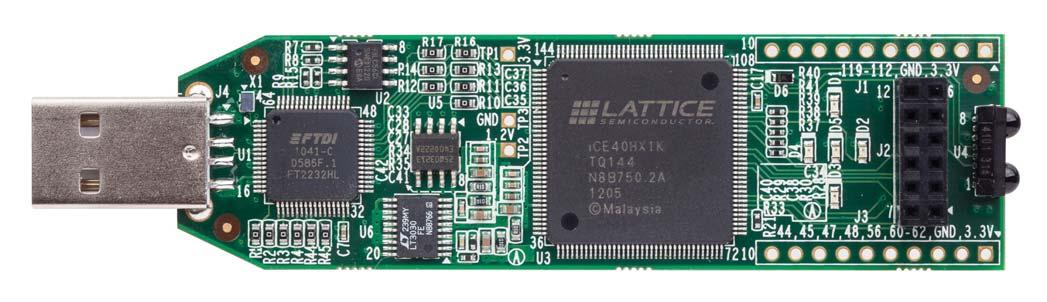
\includegraphics[width=0.8\textwidth]{iCEstick.jpg}
\end{center}

Connect to the SwapForth board using a terminal program of your choice.
Set the serial parameters to:
\begin{itemize}
\item 115200 baud
\item 8 data bits, no parity, no stop bit (often called ``8N1'', and often the default)
\end{itemize}

\begin{framed}
\begin{Verbatim}[commandchars=\\\{\}]
----------------------------------------------------------
swapForth v0.1
\end{Verbatim}
\end{framed}


%%%%%%%%%%%%%%%%%%%%%%%%%%%%%%%%%%%%%%%%%%%%%%%%%%%%%%%%%%%%%%%%%%%%%%%%

\newcommand{\worddef}[3]{
% \begin{samepage}
\vspace{1pt}
\noindent \word{#1} \mach{#2} #3
}

\newcommand{\longworddef}[3]{
\begin{samepage}
\vspace{1pt}

\noindent \word{#1}

\vspace{4pt}

\mach{#2}

\vspace{4pt}

\setlength{\parindent}{0cm}

#3

\end{samepage}

\noindent
\textcolor{lightgray}{\rule{\textwidth}{1pt}}
}

\chapter{Available Words}

\section{ANS Core Words}

J1a SwapForth implements most, but not all, of the core ANS 94 Forth standard.

\section{Additional Words}

\chapter{The SwapForth Shell}

\section{Command reference}
\section{Notes on Tethered Mode}

\chapter{Memory}

\section{RAM Types}

The J1a implementation uses 8Kbytes of RAM in a split configuration.

The lower 4K is for code.
This RAM is writable, and executable, but not (directly) readable.
The variable \mach{CP} (code pointer) points into this area.
To read from this region, use the special word \mach{code@}.

The upper 4K is for data.
This RAM is writable and readable.
The dictionary and all variables are located in this section.
The variable \mach{DP} points into this area.

\section{Dictionary Layout}

The SwapForth dictionary is a linked list;
the variable \mach{forth} holds the start of this list.
Each dictionary entry contains:

\begin{itemize}
\item \textbf{next pointer} - address of the next dictionary entry, or zero for the last dictionary entry
\item \textbf{imm} - immediate bit
\item \textbf{count} - length of the name, in characters, 1-31
\item \textbf{name$_1$ - name$_n$} - characters in name. If the length of the name is even, then a padding byte is appended
\item \textbf{xt} - execution token for the word
\end{itemize}

\vspace{10pt}
\noindent
\begin{bytefield}[endianness=big, bitwidth=2.0em]{16}
  \bitheader{0-15} \\
    \bitbox{15}{next pointer} & \bitbox{1}{\small{imm}} \\
    \bitbox{8}{name$_1$} & \bitbox{8}{count} \\
    \bitbox{16}{...} \\
    \bitbox{8}{name$_n$} & \bitbox{8}{name$_{n-1}$} \\
    \bitbox{16}{xt} \\
\end{bytefield}

\chapter{iCEstick Hardware interface}

\begin{center}
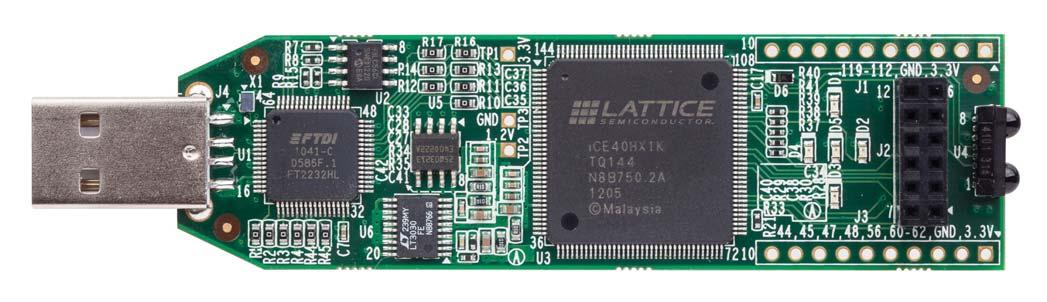
\includegraphics[width=0.8\textwidth]{iCEstick.jpg}
\end{center}

The J1a for iCEstick includes connections to the iCEstick peripherals:
\begin{itemize}
\item SPI flash
\item LEDs
\item IrDA tranceiver
\item Pmod connector
\item prototyping connectors
\item UART
\end{itemize}

Access to peripherals is via the
\mach{io@} and \mach{io!} words.
Peripherals are port-mapped into a 16-bit IO address space.

Most ports are either read-only or write-only.
For read-only ports, writing to the port has no effect.
For write-only ports, reading from the port gives zero.

As an example of direct port access, this word
blinks the on-board LEDs when a signal on IrDA is detected.

\begin{framed}
\begin{Verbatim}
: x
  begin
    $2000 io@     \ read from input port
    8 and 0=      \ true if bit 3 (IrDA RXD) is 0
    $0004 io!     \ write to LEDS
  again
;
\end{Verbatim}
\end{framed}

\section{Port Map}
\subsection{\$0001: Pmod data}

Not yet implemented.

\subsection{\$0002: Pmod direction}

Not yet implemented.

\subsection{\$0008: PIO output}

%  assign {PIO1_20, PIO1_18, PIOS_00, PIOS_02, PIOS_03} = PIOS;

Write-only port \$0008 controls the flash and IrDA outputs.

\vspace{10pt}
\noindent
\begin{bytefield}[endianness=big, bitwidth=2.0em]{16}
  \bitheader{0-15} \\
    \bitbox{11}{} &
    \bitbox{1}{\tiny{IrDA\\SD}} &
    \bitbox{1}{\tiny{IrDA\\TXD}} &
    \bitbox{1}{\tiny{flash\\SCK}} &
    \bitbox{1}{\tiny{flash\\MOSI}} &
    \bitbox{1}{\tiny{flash\\CS}}
\end{bytefield}


\subsection{\$0004: LEDs}

The five on-board LEDS are controlled by write-only port at address \$0004.
Setting a bit to 1 lights the corresponding LED.

\vspace{10pt}
\noindent
\begin{bytefield}[endianness=big, bitwidth=2.0em]{16}
  \bitheader{0-15} \\
    \bitbox{11}{} &
    \bitbox{1}{\tiny{LED5}} &
    \bitbox{1}{\tiny{LED4}} &
    \bitbox{1}{\tiny{LED3}} &
    \bitbox{1}{\tiny{LED2}} &
    \bitbox{1}{\tiny{LED1}}
\end{bytefield}

\subsection{\$1000: UART data}

\subsection{\$2000: IrDA, flash and UART inputs}

Read-only port \$2000 contains the input signals from the
IrDA receiver, SPI flash, and UART.

\vspace{10pt}
\noindent
\begin{bytefield}[endianness=big, bitwidth=2.0em]{16}
  \bitheader{0-15} \\
    \bitbox{12}{} &
    \bitbox{1}{\tiny{IrDA\\RXD}} &
    \bitbox{1}{\tiny{flash\\MISO}} &
    \bitbox{1}{\tiny{UART\\key?}} &
    \bitbox{1}{\tiny{UART\\busy}}
\end{bytefield}

\clearpage
\addcontentsline{toc}{chapter}{Index}
\printindex

\end{document}
